\scanpage{85}
% archive sheet number: 84
% Three large diagonal cancellation strokes cross the typescript.
\deleted{\uline{Remarks} \raisebox{2ex}{\inserted{\handwritten{4}}} a) One should beware of believing that when $A$ is a n\unsure{\rlap{e}o|o}et\rlap{é}h\rlap{h}erian ring, $B$ a flat $A$-algebra of finite type, $(J_i)_{i\quad I}$ a family of ideals of $A$ whose intersection is zero, then the intersection of the $J_iB$ is zero. (We have already pointed out the example of a discrete valuation ring $A$, equipped with the \mbox{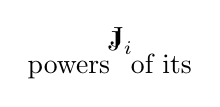
\begin{tikzpicture}[baseline=(left.base)]
\node[inner sep=0] (left) {powers};
\node[anchor=base west,inner sep=0,xshift=.25cm] at (left.base east) {of its};
\node[anchor=south west,inner sep=0,xshift=-.05cm,yshift=.08cm] at (left.north east) {\inserted{$\text{\rlap{J}\raisebox{.3ex}{\kern.08em J}}_i$}};
\end{tikzpicture}} maximal ideal, and $B$ being the field of fractions). \deleted{The fact} Indeed, the hypothesis that $\quad J_i=0$ does not at all imply that $\quad J_i=0$ !}

\deleted{b) Let $X$ be a prescheme over a field $k$, and let $u_i\colon Z_i\quad X$ be a schematically dominant family. We do not know whether for every base change $S\quad\operatorname{Spec}(k)$, the family of the $u_{i\,S}\colon Z_{i\,S}\quad X_S$ is schematically \mbox{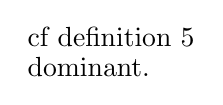
\begin{tikzpicture}[baseline=(base.base)]
\node[inner sep=0] (base) {dominant.};
\node[anchor=south west,inner sep=0,yshift=.12cm] at (base.north west) {\inserted{cf definition 5}};
\end{tikzpicture}} One can \deleted{reduce} show (by arguments of the type of those used below) that for this it suffices that this property be satisfied whenever $S$ is the spectrum of a field $k'$ a finite separable extension of $k$. On the other hand, we shall see below that the answer is affirmative when $X$ is locally noetherian.}

\deleted{\uline{Definition} 5. With the notation of 1., suppose that $X$ is an $S$-prescheme. We say that $(u_i)$ is \deleted{relatively} schematically dominant relative to $S$ \deleted{(or that the family of subpreschemes $Z_i$, if they are such, is schematically dense in $X$ relative to $S$)} if for every $S'\quad S$, the family of the $u_{i\,S'}\colon Z_{i\,S'}\quad X_{S'}$ is schematically dominant \deleted{(resp or that the family} When the $Z_i$ are subpreschemes of $X$ \ldots, we also say that the family \deleted{of the} $\unsure{(Z_i)|\{Z_i)}$ is schematically dense in $X$ relative to $S$.}

\deleted{NB This is a local notion on $X$ and on $S$.}

\deleted{\uline{Lemma} 6\quad With the preceding notation, suppose $X$ and the $Z_i$ flat over $S$, let $S_o$ be a subprescheme of $S$ defined by a Nilpotent Ideal. If the family of the $u_{i\,S_o}$ is schematically dominant, the same holds for the family of the $u_i$. One can resper with ``relative to $S$''.}

\deleted{The second assertion follows trivially from the first and the definitions. For the first, cf SGAD IX. 4.2.}
